\subsection{Apparato A}

% Doveva farlo Bob.

\subsubsection{Descrizione del circuito}

Il circuito del primo apparato costruito è rappresentato in \autoref{circuitone}.

\begin{figure}[h]
\centering
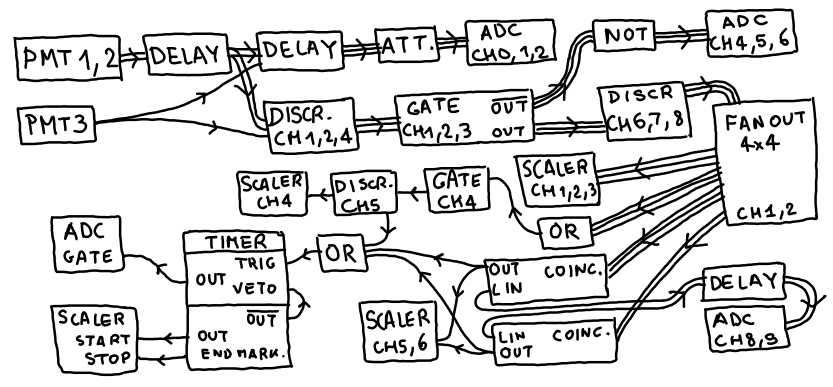
\includegraphics[width=30 em]{immagini/circuitone}
\caption{Schema circuitale dell'apparato A.}
\label{circuitone}
\end{figure}

Le uscite dei PMT sono inviate ai discriminatori, le cui uscite attraversano un modulo di antiretrigger (tempo morto di \SI{1}{\micro s}) e vengono usate per costruire funzioni logiche. I segnali dei PMT vengono anche inviati all'ADC attraverso un attenuatore per evitare di danneggiare lo strumento.
Per quanto riguarda la parte logica, costruiamo e mettiamo in tempo tre tipi di trigger:
\begin{enumerate}
\item canale
\item coincidenza a 2
\item coincidenza a 3.
\end{enumerate}
Il trigger di canale è semplicemente il segnale discriminato del PMT corrispondente; quello di coincidenze è dato dall'uscita di lunga durata del modulo stesso. Mandiamo questi segnali all'ADC in modo che il trigger di canale arrivi in contemporanea con il segnale analogico del canale stesso. Se in quel momento c'è anche un trigger di coincidenza, sappiamo se l'evento ci è arrivato da una coincidenza anziché da un canale singolo. Abbiamo fatto tutto questo per acquisire tutti i canali contemporaneamente ed agevolare la lettura dei dati via software. Purtroppo il \emph{cross-talk}%
\footnote{Spiegheremo come ci siamo accorti di questo problema nella \autoref{ref}.} presente nell'ADC ha rovinato le misure fatte con questo apparato.
Per dare precedenza agli eventi più rari abbiamo collegato questi trigger ad un modulo \emph{or} ritardando i trigger singoli rispetto a quelli di coincidenze a 2 e questi ultimi rispetto alle coincidenze a 3. L'uscita dell'\emph{or} era poi inviata ad un \emph{timer} che generava il gate dell'ADC. L'altro canale di questo \emph{timer} veniva usato per avviare o fermare le acquisizioni.

\subsubsection{Problemi riscontrati}

I problemi descritti in seguito ci hanno spinti a semplificare il circuito per cercare di risolverli.

Il più evidente fin da subito è stato il \emph{bit stuck}: il terzo bit dei dati in formato binario è sempre 1. Gli istogrammi presentano delle lacune di \SI{4}{digit} ogni \SI{4}{digit}. Risolviamo questo problema istogrammando con canali più larghi di \SI{8}{digit}.

Poi abbiamo escluso l'\emph{or} dal circuito perché i segnali che ci arrivavano dalle coincidenze mostravano avere un'energia minore. Abbiamo risolto il problema togliendo l'\emph{or} dal circuito.

Il problema più interessante è dato dal fatto che, confrontando gli spettri del \na{}, abbiamo visto che i fotoni emessi dalla sorgente con attività maggiore avevano energia maggiore.
Il grafico in \autoref{distanze} mostra l'energia dei fotopicchi del sodio in funzione della distanza della sorgente ad attività elevata dal rivelatore usato per fare la misura.
\marginpar{Sto supponendo che prima di questo punto abbiamo scritto che ci sono due sorgenti di sodio.}